\documentclass[11pt]{article}
\usepackage[margin=1in]{geometry}
\usepackage{amsmath,amssymb}
\usepackage{graphicx}
\usepackage{booktabs}
\usepackage{natbib}
\usepackage[hidelinks]{hyperref}
\usepackage{xcolor}
\usepackage{framed}

% Written by make_figures.py; do not edit.
\newcommand{\CaseCentredRawAnchorCosIdx}{161}
\newcommand{\CaseCentredRawAnchorCosPass}{56\%}
\newcommand{\CaseCentredRawAnchorEucIdx}{189}
\newcommand{\CaseCentredRawAnchorEucPass}{55\%}
\newcommand{\CaseCentredRawAnchorInter}{+0.035}
\newcommand{\CaseCentredRawAnchorP}{4e-15}
\newcommand{\CaseCentredRawGatedCosIdx}{138}
\newcommand{\CaseCentredRawGatedCosPass}{61\%}
\newcommand{\CaseCentredRawGatedEucIdx}{160}
\newcommand{\CaseCentredRawGatedEucPass}{58\%}
\newcommand{\CaseCentredRawGatedInter}{+0.015}
\newcommand{\CaseCentredRawGatedP}{0.025}
\newcommand{\CaseCentredRunAnchorCosIdx}{161}
\newcommand{\CaseCentredRunAnchorCosPass}{54\%}
\newcommand{\CaseCentredRunAnchorEucIdx}{189}
\newcommand{\CaseCentredRunAnchorEucPass}{55\%}
\newcommand{\CaseCentredRunAnchorInter}{+0.034}
\newcommand{\CaseCentredRunAnchorP}{5.7e-15}
\newcommand{\CaseCentredRunGatedCosIdx}{143}
\newcommand{\CaseCentredRunGatedCosPass}{58\%}
\newcommand{\CaseCentredRunGatedEucIdx}{160}
\newcommand{\CaseCentredRunGatedEucPass}{58\%}
\newcommand{\CaseCentredRunGatedInter}{+0.013}
\newcommand{\CaseCentredRunGatedP}{0.046}
\newcommand{\CaseCentredTzeroAnchorCosIdx}{167}
\newcommand{\CaseCentredTzeroAnchorCosPass}{34\%}
\newcommand{\CaseCentredTzeroAnchorEucIdx}{189}
\newcommand{\CaseCentredTzeroAnchorEucPass}{55\%}
\newcommand{\CaseCentredTzeroAnchorInter}{+0.032}
\newcommand{\CaseCentredTzeroAnchorP}{4.2e-14}
\newcommand{\CaseCentredTzeroGatedCosIdx}{163}
\newcommand{\CaseCentredTzeroGatedCosPass}{32\%}
\newcommand{\CaseCentredTzeroGatedEucIdx}{160}
\newcommand{\CaseCentredTzeroGatedEucPass}{58\%}
\newcommand{\CaseCentredTzeroGatedInter}{+0.003}
\newcommand{\CaseCentredTzeroGatedP}{0.6}
\newcommand{\CaseUnitRawAnchorCosIdx}{147}
\newcommand{\CaseUnitRawAnchorCosPass}{100\%}
\newcommand{\CaseUnitRawAnchorEucIdx}{189}
\newcommand{\CaseUnitRawAnchorEucPass}{55\%}
\newcommand{\CaseUnitRawAnchorInter}{+0.038}
\newcommand{\CaseUnitRawAnchorP}{8.6e-18}
\newcommand{\CaseUnitRawGatedCosIdx}{124}
\newcommand{\CaseUnitRawGatedCosPass}{100\%}
\newcommand{\CaseUnitRawGatedEucIdx}{160}
\newcommand{\CaseUnitRawGatedEucPass}{58\%}
\newcommand{\CaseUnitRawGatedInter}{+0.018}
\newcommand{\CaseUnitRawGatedP}{0.0097}
\newcommand{\CaseUnitRunAnchorCosIdx}{187}
\newcommand{\CaseUnitRunAnchorCosPass}{53\%}
\newcommand{\CaseUnitRunAnchorEucIdx}{189}
\newcommand{\CaseUnitRunAnchorEucPass}{55\%}
\newcommand{\CaseUnitRunAnchorInter}{+0.020}
\newcommand{\CaseUnitRunAnchorP}{1.7e-08}
\newcommand{\CaseUnitRunGatedCosIdx}{478}
\newcommand{\CaseUnitRunGatedCosPass}{57\%}
\newcommand{\CaseUnitRunGatedEucIdx}{160}
\newcommand{\CaseUnitRunGatedEucPass}{58\%}
\newcommand{\CaseUnitRunGatedInter}{-0.057}
\newcommand{\CaseUnitRunGatedP}{1.2e-12}
\newcommand{\CaseUnitTzeroAnchorCosIdx}{174}
\newcommand{\CaseUnitTzeroAnchorCosPass}{72\%}
\newcommand{\CaseUnitTzeroAnchorEucIdx}{189}
\newcommand{\CaseUnitTzeroAnchorEucPass}{55\%}
\newcommand{\CaseUnitTzeroAnchorInter}{+0.026}
\newcommand{\CaseUnitTzeroAnchorP}{1.9e-11}
\newcommand{\CaseUnitTzeroGatedCosIdx}{363}
\newcommand{\CaseUnitTzeroGatedCosPass}{72\%}
\newcommand{\CaseUnitTzeroGatedEucIdx}{160}
\newcommand{\CaseUnitTzeroGatedEucPass}{58\%}
\newcommand{\CaseUnitTzeroGatedInter}{-0.037}
\newcommand{\CaseUnitTzeroGatedP}{6.3e-07}
\newcommand{\CentredCosMax}{50\%}
\newcommand{\CentredCosMin}{50\%}
\newcommand{\CentredEucEight}{0.5\%}
\newcommand{\CentredEucTwo}{48\%}
\newcommand{\DiagAllCos}{124}
\newcommand{\DiagAllEuc}{162}
\newcommand{\DiagFixCosHi}{78}
\newcommand{\DiagFixCosLo}{77}
\newcommand{\DiagFixEucHi}{134}
\newcommand{\DiagFixEucLo}{124}
\newcommand{\DiagOrigCos}{78}
\newcommand{\DiagOrigEuc}{134}
\newcommand{\DiagTrustCos}{117}
\newcommand{\DiagTrustEuc}{169}
\newcommand{\DriftCos}{33\%}
\newcommand{\DriftEuc}{62\%}
\newcommand{\MatchCentredAng}{0.95}
\newcommand{\MatchCentredCos}{0.42}
\newcommand{\MatchCentredEuc}{1.01}
\newcommand{\MatchUnitAng}{0.36}
\newcommand{\MatchUnitCos}{0.07}
\newcommand{\MatchUnitEuc}{0.51}
\newcommand{\MinCells}{18}
\newcommand{\MinCosAngPassDiff}{0.006}
\newcommand{\MinCosAngVarDiff}{0.00}
\newcommand{\MinRawGroupClose}{42\%}
\newcommand{\MinRawGroupGap}{0.68}
\newcommand{\MinRawGroupGapMax}{7.1}
\newcommand{\MinRawPassGap}{0.19}
\newcommand{\MinRawVarGap}{1.32}
\newcommand{\MinRawVarGapMax}{+2.72}
\newcommand{\MinRawVarGapMin}{-6.49}
\newcommand{\MinRunGroupClose}{83\%}
\newcommand{\MinRunGroupGap}{0.08}
\newcommand{\MinRunGroupGapMax}{3.7}
\newcommand{\MinRunPassGap}{0.01}
\newcommand{\MinRunVarGap}{0.61}
\newcommand{\MinRunVarGapMax}{+2.58}
\newcommand{\MinRunVarGapMin}{+0.02}
\newcommand{\MinTzeroGroupClose}{33\%}
\newcommand{\MinTzeroGroupGap}{0.78}
\newcommand{\MinTzeroGroupGapMax}{4.9}
\newcommand{\MinTzeroPassGap}{0.16}
\newcommand{\MinTzeroVarGap}{1.18}
\newcommand{\MinTzeroVarGapMax}{+3.41}
\newcommand{\MinTzeroVarGapMin}{+0.02}
\newcommand{\UnitFourAng}{32\%}
\newcommand{\UnitFourCos}{94\%}
\newcommand{\UnitFourEuc}{14\%}
\newcommand{\UnitSixteenCos}{99.7\%}
\newcommand{\UnitSixteenEuc}{0.0\%}
   % every number in the text, written by make_figures.py

\title{One Threshold, Different Rules: How an Unmatched Confidence Bound Manufactures Geometry Effects in Bounded-Confidence Models}
\author{Krishnasai Addala\\ \small Independent researcher}
\date{Draft, \today}

\begin{document}
\maketitle

\begin{abstract}
Multidimensional bounded-confidence models increasingly compare distance measures: Euclidean, cosine, angular and others.
A common way to do so is to run each metric at the same numerical confidence bound $\varepsilon$.
We show that this compares different interaction rates, not different geometries.
For uniform opinions, the share of pairs a gate admits at one $\varepsilon$ differs between metrics by large factors that depend on where the opinion space is centred and on its dimension; in the unit cube $[0,1]^4$ at $\varepsilon=0.5$, \UnitFourEuc\ of pairs pass a Euclidean gate and \UnitFourCos\ pass a cosine gate.
In a minimal Deffuant model, a shared bound produces large apparent geometry effects on the interaction rate and the number of opinion groups.
Matching bounds on the share of pairs admitted at the start does not remove them, because that share drifts apart during the run; matching on the share admitted over the whole run does, leaving only a variance difference that comes from the angular update rule rather than the gate.
Cosine and angular gates are monotone transforms of each other and, once matched, behave as one.
In an agent-based model of AI governance, an unpublished draft reported that geometry reverses the effect of enforcement lag on shocks.
Working forward from the corrected model and backward from the original, we show that the shared threshold made the two geometries' effects differ greatly in size, while the reversal itself came from trust shrinking each agent's perceived policy toward the origin, which in the uncentred space meant ``no regulation at all''.
We give a five-point reporting protocol for any study that compares distance measures.
\end{abstract}

\section{Introduction}

Bounded-confidence (BC) models of opinion dynamics let two agents influence each other only when their opinions are close enough \citep{deffuant2000,hegselmann2002}.
With one-dimensional opinions, ``close enough'' has an obvious meaning.
With several dimensions it does not, and the choice of distance has become a modelling decision in its own right.
Euclidean distance is the default for multidimensional BC models \citep{lorenz2008}, but angular distances \citep{schweighofer2020}, $L_1$ and $L_\infty$ norms, and topic-weighted discordances \citep{li2026} have all been proposed, often with the argument that the choice changes what the model predicts.

A comparison between two distance measures needs a confidence bound for each.
The simplest choice, and the one most easily made without noticing, is the same number for both.
This paper argues that a shared bound confounds two things: \emph{which} pairs a metric treats as close (its shape), and \emph{how many} pairs it lets interact (its size).
The second is often much larger than the first.
\citet{li2026} note exactly this in passing: in their model, lowering the topic weight at a fixed bound enlarges the region of opinions an agent will listen to, and they attribute the resulting change in fragmentation to ``the larger size and non-square shape'' of that region together.
Separating the two requires holding size fixed.

We make the argument in three steps.
Section~\ref{sec:coverage} shows, with no simulation, how far the share of interacting pairs at one $\varepsilon$ differs between Euclidean, cosine and angular distance, and how this depends on centring and dimension.
Section~\ref{sec:minimal} uses a minimal Deffuant model to show what a shared bound does to conclusions, and how much of the apparent geometry effect survives when bounds are matched, either at the start of a run or over the whole run.
The second matters: coverage matched at the start drifts apart as opinions move.
Section~\ref{sec:case} is a case study: an agent-based model of AI governance in which we reported that the geometry of the opinion space reverses the effect of enforcement lag on shocks.
We found in our own audit, before publication, that the finding was not a property of geometry; two complementary reruns show that the shared threshold changed the size of the effects and that an origin-dependent step elsewhere in the model flipped their sign.
Section~\ref{sec:protocol} turns the lessons into a short reporting protocol.

\section{Background: what $\varepsilon$ means under each metric}
\label{sec:background}

We consider opinions $x_i \in \mathbb{R}^d$ and three distances:
\begin{align*}
d_{\mathrm{E}}(x_i,x_j) &= \lVert x_i - x_j \rVert_2, \\
d_{\cos}(x_i,x_j) &= 1 - \frac{x_i \cdot x_j}{\lVert x_i\rVert\,\lVert x_j\rVert}, \\
d_{\angle}(x_i,x_j) &= \arccos \frac{x_i \cdot x_j}{\lVert x_i\rVert\,\lVert x_j\rVert}.
\end{align*}
Two agents may interact when $d(x_i,x_j) \le \varepsilon$.
The units of $\varepsilon$ differ: a length for $d_{\mathrm{E}}$, a number in $[0,2]$ for $d_{\cos}$, and an angle in $[0,\pi]$ for $d_\angle$.
The same number therefore means different things: $d_{\cos} \le 0.5$ admits angles up to $60^\circ$, $d_\angle \le 0.5$ admits angles up to $28.6^\circ$.
The angular metrics also depend on where the origin is.
If opinions are coded in $[0,1]^d$, every opinion vector points into the positive orthant and no two are more than $90^\circ$ apart, so an angular gate measures direction as seen from the corner where every dimension is at its minimum, not ideological direction.
Coding opinions in $[-1,1]^d$ with $0$ as neutral makes the angle a measure of alignment.

Because $d_{\cos} = 1 - \cos d_\angle$ is strictly increasing in $d_\angle$, a cosine gate at $\varepsilon$ and an angular gate at $\arccos(1-\varepsilon)$ admit exactly the same pairs.
Once their bounds are matched, the two metrics can differ only through their update rules.

The updates we use move agent $i$ a fraction $r$ of the way toward agent $j$: a straight-line step for Euclidean distance; for the angular metrics, a step of $i$'s direction toward $j$'s (along the chord for cosine, along the great circle for angular distance) that keeps $i$'s magnitude.

\section{How many pairs does one threshold admit?}
\label{sec:coverage}

Before any dynamics, a gate has a \emph{coverage}: the share of pairs it admits.
For opinions drawn independently and uniformly, which is how most BC studies start, coverage at the first step is the same for network-neighbour pairs as for random pairs, and it can be computed directly.
Figure~\ref{fig:coverage} shows it for $d=4$ in both opinion spaces, and Table~\ref{tab:coverage} for $d$ from 2 to 16.

\begin{figure}[t]
\centering
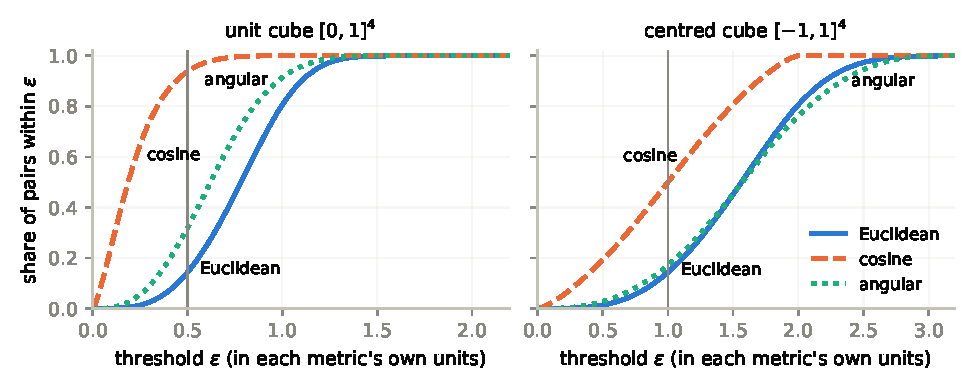
\includegraphics[width=\linewidth]{figures/fig1_coverage.pdf}
\caption{Share of uniformly drawn pairs within $\varepsilon$, for $d=4$. Vertical lines mark the conventional bounds, $0.5$ in the unit cube and the equivalent $1.0$ in the centred cube. Each metric's $\varepsilon$ is in its own units, so a shared value picks out a different point on each curve. Monte Carlo with $2\times10^5$ pairs; checked against a deterministic quadrature in $d=2$ at $\varepsilon=0.4$, where they agree to within one percentage point.}
\label{fig:coverage}
\end{figure}

\begin{table}[t]
\centering
\small
\begin{tabular}{llrrrr}
\toprule
space & $\varepsilon$ & $d$ & Euclidean & cosine & angular \\
\midrule
unit & 0.5 & 2 & 48\% & 92\% & 58\% \\
unit & 0.5 & 4 & 14\% & 94\% & 32\% \\
unit & 0.5 & 8 & 1\% & 98\% & 15\% \\
unit & 0.5 & 16 & 0\% & 100\% & 4\% \\
centred & 1 & 2 & 48\% & 50\% & 32\% \\
centred & 1 & 4 & 14\% & 50\% & 17\% \\
centred & 1 & 8 & 1\% & 50\% & 7\% \\
centred & 1 & 16 & 0\% & 50\% & 1\% \\
\bottomrule
\end{tabular}

\caption{Share of uniformly drawn pairs admitted at one shared $\varepsilon$, by opinion space and dimension.}
\label{tab:coverage}
\end{table}

Three things stand out.
First, in the unit cube a cosine gate barely restricts anything: at $\varepsilon = 0.5$ it admits \UnitFourCos\ of pairs in four dimensions, against \UnitFourEuc\ for Euclidean distance, and the gap widens with dimension (\UnitSixteenCos\ against \UnitSixteenEuc\ at $d=16$).
All opinion vectors lie in the positive orthant, so the angles between them are small.
Second, centring changes this, but does not make one number mean the same thing everywhere.
In the centred cube, a cosine gate at $\varepsilon = 1$ admits pairs less than $90^\circ$ apart, which by symmetry is half of all pairs in every dimension (\CentredCosMin\ at each $d$ in Table~\ref{tab:coverage}); a Euclidean gate at the same value admits \CentredEucTwo\ of pairs at $d=2$ and \CentredEucEight\ at $d=8$, because distances grow with dimension while angles do not.
Third, the thresholds that do give equal coverage look nothing alike.
To admit 15\% of pairs in $[0,1]^4$, Euclidean distance needs $\varepsilon = \MatchUnitEuc$, cosine $\MatchUnitCos$ and angular $\MatchUnitAng$; in $[-1,1]^4$ the values are \MatchCentredEuc, \MatchCentredCos\ and \MatchCentredAng.

A study that runs every metric at one $\varepsilon$ is therefore comparing interaction rates that differ by a factor that depends on the coding of the space and on its dimension.
The rest of the paper asks how much this matters once the dynamics run.

\section{A minimal model}
\label{sec:minimal}

\subsection{Model}
$n=500$ agents sit on an Erd\H{o}s--R\'enyi graph with mean degree 10; opinions start uniform in $[0,1]^d$ (the \emph{unit} space) or $[-1,1]^d$ (the \emph{centred} space), for $d \in \{2,4,8\}$.
Each round draws a random matching of the graph's edges, so no agent takes part in two conversations in a round.
For every matched pair within $\varepsilon$, both agents move a fraction $\mu=0.3$ toward the other's previous opinion under the metric's update rule \citep{deffuant2000}, and are clipped back into the cube.
Runs last 2{,}000 rounds.
A seed fixes the graph, the initial opinions and the sequence of matchings, so runs with the same seed differ only in the gate and the update rule.
The model is described in ODD format \citep{grimm2020} in Appendix~\ref{app:odd}.

\subsection{Threshold rules}
In each cell (space, dimension, reference coverage) Euclidean distance runs at the $\varepsilon$ that admits a share $c \in \{5\%, 15\%, 30\%\}$ of pairs at the start.
Cosine and angular distance each run under three rules:
\begin{description}
\item[raw:] the same number as the Euclidean $\varepsilon$;
\item[matched at $t=0$:] the $\varepsilon$ that admits the same share $c$ of pairs at the start;
\item[matched over the run:] the $\varepsilon$ whose pass rate, averaged over the whole run, equals the Euclidean run's (found by bisection on ten pilot seeds that are not reused).
\end{description}
Because initial opinions are independent of the graph, the share of random pairs and the share of neighbour pairs within $\varepsilon$ coincide at $t=0$.

\subsection{Outcomes}
Final opinion variance (mean over dimensions); directional dispersion, $1 - \lVert \overline{x/\lVert x \rVert} \rVert$; the number of opinion groups holding at least 1\% of agents, where a group is a connected set of final opinions within $0.1\varepsilon$ of each other under the run's metric; the effective number of groups, $1/\sum_k s_k^2$ over group shares $s_k$; and the realised pass rate, the share of matched pairs within $\varepsilon$ over the whole run.
Each cell has 100 seeds, paired across metrics and rules.

\subsection{Results}

Figure~\ref{fig:minimal} shows, for each of the \MinCells\ cells and both angular metrics, the paired gap to the Euclidean run under each threshold rule.
Pass rates are compared as differences; variance and the effective number of groups as $\log_2$ ratios, so a gap of 1 means twice Euclidean's value.
With 100 paired seeds almost every gap differs significantly from zero, so we report sizes.

\begin{figure}[t]
\centering
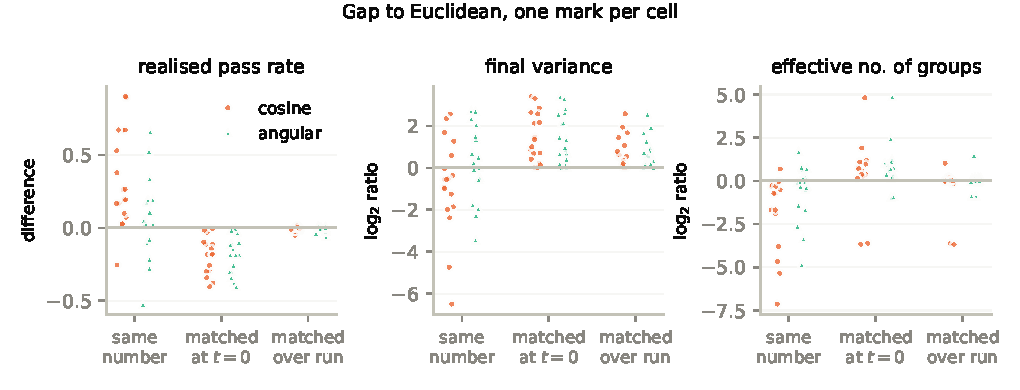
\includegraphics[width=\linewidth]{figures/fig2_minimal_gaps.pdf}
\caption{Paired gap between each angular metric and Euclidean distance, by threshold rule. One mark per cell (space $\times$ dimension $\times$ reference coverage), mean over 100 seeds. Left: realised pass rate (difference). Middle and right: final variance and effective number of opinion groups ($\log_2$ ratio).}
\label{fig:minimal}
\end{figure}

\paragraph{A shared bound changes the interaction rate, and the conclusions with it.}
Under one shared $\varepsilon$, the realised pass rate differs from Euclidean's by a median of \MinRawPassGap\ (as a share of attempted interactions), and the effective number of groups by a median factor of $2^{\MinRawGroupGap}$, reaching $2^{\MinRawGroupGapMax}$ in the unit cube, where a cosine gate admits nearly every pair and the population collapses to one group.
Read naively, these are large geometry effects.

\paragraph{Matching at the start is not enough.}
Matching coverage at $t=0$ equalises the share of pairs that \emph{can} interact at the start, but not over the run: the median pass-rate gap is still \MinTzeroPassGap, and the median group-count gap is \MinTzeroGroupGap\ on the $\log_2$ scale, no smaller than under a shared bound.
The reason is visible in the left panel.
Coverage evolves with the dynamics: as agents converge, more of their pairs fall within $\varepsilon$, and in every cell the realised pass rate ends above the starting coverage.
It climbs further under Euclidean distance than under the angular metrics (for example, from 15\% at the start to \DriftEuc\ over the run against \DriftCos\ for cosine, in the centred cube with $d=4$).
One plausible reason is that angular updates rotate an opinion but keep its length, so they close only part of the distance between two agents.
Matching at the start fixes the initial value of a quantity that then drifts apart.

\paragraph{Matching over the run removes the interaction gap.}
When each angular bound is chosen so that its pass rate over the whole run equals Euclidean's, the median pass-rate gap falls to \MinRunPassGap, and the group structure follows: the median group-count gap is \MinRunGroupGap, and \MinRunGroupClose\ of cases end within a factor of $2^{0.5}$ of Euclidean's group count (against \MinRawGroupClose\ under a shared bound).
The exceptions all have the lowest reference coverage (5\%) and low dimension, where the matched bounds are very small (cosine $\varepsilon$ of 0.001 to 0.2) and the group structure after 2{,}000 rounds is still far from settled.

\paragraph{What remains is the update rule.}
A variance gap survives every matching rule (median \MinRunVarGap\ on the $\log_2$ scale when matched over the run, ranging from \MinRunVarGapMin\ to \MinRunVarGapMax).
This is a genuine geometric difference, and its likely source is that the angular updates move an agent's direction but keep its distance from the origin, so agents can agree in direction while remaining spread out in magnitude.
It belongs to the update rule, not to the gate, which is exactly the separation a matched comparison is meant to make.

\paragraph{Cosine and angular gates are one gate.}
Matched at $t=0$, the cosine and angular runs' realised pass rates never differ by more than \MinCosAngPassDiff, and their median variance gaps to Euclidean differ by \MinCosAngVarDiff.
Cosine distance is a monotone function of the angle, so once matched the two gates admit the same pairs, and their remaining difference (chordal versus geodesic steps) is negligible here.

\section{Case study: a geometry ``reversal'' in a model of AI governance}
\label{sec:case}

\subsection{The model and the claim}
PolicySwarm is an agent-based model of how a population's views on AI regulation respond to a policy, to media and to shocks.
Agents hold four-dimensional opinions (deployment caps, transparency, enforcement, audit intensity) on a Barab\'asi--Albert network; each tick combines bounded-confidence peer influence, a media pull, random shocks to some agents, and a pull toward the policy that each agent perceives.
Its Experiment~4 estimates how much a schedule of shocks changes the final variance of opinions, comparing paired runs with and without shocks, and asks how this effect depends on enforcement lag.

An earlier draft of our paper reported that geometry \emph{reverses} this dependence: as lag rose from 0 to 40 ticks, the shock effect grew under Euclidean distance (indexed 100, 101, 143) and shrank under cosine distance (100, 92, 72).\footnote{These are the draft's reported figures. The saved results of the corresponding $S=30$ run give 100, 97, 131 and 100, 92, 75: the same pattern, slightly different values.}
We did not publish it.
A code audit replaced it with a model in which both geometries amplify, and listed several changes, two of them about the gate:
\begin{enumerate}
\item \textbf{A shared, uncentred threshold.} Opinions were coded in $[0,1]^4$ and both metrics used $\varepsilon = 0.5$, so the gate admitted about \UnitFourEuc\ of pairs under Euclidean distance and \UnitFourCos\ under cosine (Section~\ref{sec:coverage}).
\item \textbf{A gated policy pull.} Agents were nudged toward the policy by $0.05\,(p - x_i)$ only after a conversation that passed the gate, so the strength of the policy pull scaled with coverage, and hence with the metric.
\end{enumerate}
It also fixed a cosine step that added a direction-space vector to an unnormalised opinion, separated the random streams used by shocks from those used by the policy pull (so paired control and treatment runs see the same noise), and moved the tick at which the policy tightens away from the largest lag.
We expected the two gate choices to explain the reversal.
They do not, and finding out what does turned out to illustrate the paper's point from a different direction.

\subsection{Design}
We ran two complementary experiments.

\paragraph{Forward: switching the gate choices on in the audited model.}
We reran Experiment~4 on the audited engine with three choices switched independently:
\emph{gate space} (unit: the gate and the angular steps act on $[0,1]$ coordinates, so angles are measured from the corner of the cube; centred: from its centre),
\emph{threshold} (shared: both metrics at Euclidean's value, 0.5 in unit coordinates or the equivalent 1.0 in centred ones; matched at $t=0$; or matched over the run, with cosine's bound calibrated on ten pilot seeds so that its realised pass rate equals Euclidean's), and
\emph{policy pull} (gated, as in the draft; or an ungated anchor applied to every agent each tick, with its rate set to the gated pull's expected rate under the Euclidean gate).
The audited engine's other mechanisms (media, shocks and the policy pull, including its trust scaling, which it applies around the neutral point) do not depend on which coordinates the gate uses; as a check, a Euclidean gate at 0.5 on unit coordinates reproduces a gate at 1.0 on centred coordinates to machine precision.
This experiment therefore isolates the gate; it cannot show effects that come from elsewhere in the model.
As in the draft, the policy pull starts at the enforcement lag.
Each of the $2 \times 3 \times 2$ corners crosses two geometries with lags $\{0, 20, 40\}$, with 100 paired seeds.

\paragraph{Backward: undoing the audit's changes in the original model.}
We also ran the original, pre-audit engine with its own settings, which reproduces the saved $S=30$ run exactly (Euclidean 131, cosine 75 at lag 40), and undid the audit's other changes one at a time: the cosine step, the random streams, and the tightening tick, in all eight combinations, with 100 seeds each.
When none of these removed the reversal, we compared the two engines' code line by line for any remaining step that is not equivariant under the change of coordinates, and found one (below), which we then switched as well.

The outcome in both experiments is the draft's own measure: the size of the mean shock effect at lag 40, indexed to lag 0 $=100$.
We also report the paired lag contrast in the relative shock effect for each geometry, and its difference between geometries, tested across seeds (Table~\ref{tab:case}).

\subsection{Results}

\begin{figure}[t]
\centering
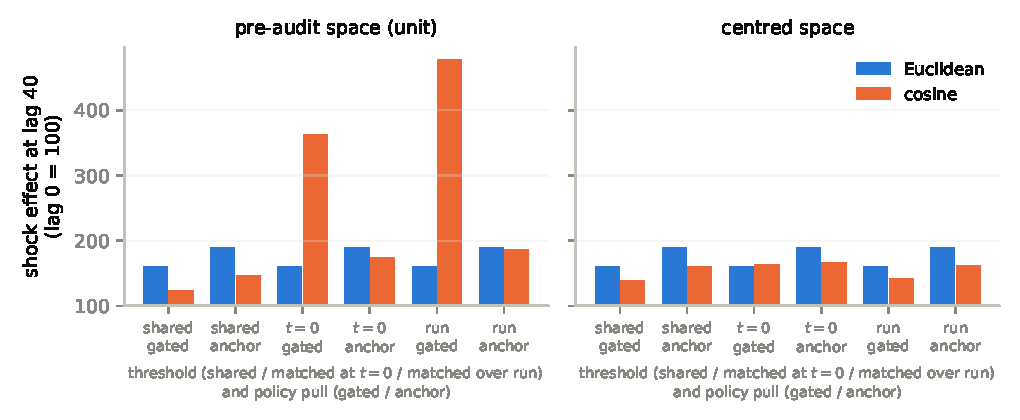
\includegraphics[width=\linewidth]{figures/fig3_case_factorial.pdf}
\caption{Experiment~4 on the audited engine with the gate-related choices switched independently. Bars give the shock effect at lag 40 relative to lag 0 ($=100$); above 100 means the effect grows with lag. 100 paired seeds per bar. No corner reproduces the draft's reversal, in which cosine fell to 72.}
\label{fig:case}
\end{figure}

\begin{table}[t]
\centering
\scriptsize
\begin{tabular}{lllrrrrl}
\toprule
space & $\varepsilon$ & pull & \multicolumn{2}{c}{pass rate (E / C)} & \multicolumn{2}{c}{lag-40 index (E / C)} & interaction [95\% CI] \\
\midrule
unit & shared & gated & 0.58 & 1.00 & 160 & 124 & +0.018 [+0.005, +0.032] \\
unit & shared & anchor & 0.55 & 1.00 & 189 & 147 & +0.038 [+0.031, +0.045] \\
unit & matched $t{=}0$ & gated & 0.58 & 0.72 & 160 & 363 & -0.037 [-0.051, -0.023] \\
unit & matched $t{=}0$ & anchor & 0.55 & 0.72 & 189 & 174 & +0.026 [+0.019, +0.033] \\
unit & matched run & gated & 0.58 & 0.57 & 160 & 478 & -0.057 [-0.071, -0.043] \\
unit & matched run & anchor & 0.55 & 0.53 & 189 & 187 & +0.020 [+0.014, +0.027] \\
centred & shared & gated & 0.58 & 0.61 & 160 & 138 & +0.015 [+0.002, +0.029] \\
centred & shared & anchor & 0.55 & 0.56 & 189 & 161 & +0.035 [+0.027, +0.042] \\
centred & matched $t{=}0$ & gated & 0.58 & 0.32 & 160 & 163 & +0.003 [-0.009, +0.016] \\
centred & matched $t{=}0$ & anchor & 0.55 & 0.34 & 189 & 167 & +0.032 [+0.024, +0.039] \\
centred & matched run & gated & 0.58 & 0.58 & 160 & 143 & +0.013 [+0.000, +0.026] \\
centred & matched run & anchor & 0.55 & 0.54 & 189 & 161 & +0.034 [+0.027, +0.042] \\
\bottomrule
\end{tabular}

\caption{The case-study factorial. Pass rates are realised gate pass rates in control runs (E: Euclidean, C: cosine). The lag-40 index is the draft's measure (lag 0 $=100$). The interaction is cosine's lag contrast in the relative shock effect minus Euclidean's, paired by seed.}
\label{tab:case}
\end{table}

\paragraph{The gate choices change the size of the effect, never its sign.}
In every corner of the forward experiment, both geometries amplify with lag (Figure~\ref{fig:case}).
The gate choices still matter a great deal for how much.
With the draft's shared threshold in the unit cube, the cosine gate passes \CaseUnitRawGatedCosPass\ of attempted conversations against \CaseUnitRawGatedEucPass\ for Euclidean, and cosine's lag-40 index is \CaseUnitRawGatedCosIdx\ against \CaseUnitRawGatedEucIdx.
Matching the threshold in the unit cube does not make the geometries agree: the matched cosine bounds are tiny, because all opinion vectors point into one orthant, and with the gated pull the cosine index swings to \CaseUnitTzeroGatedCosIdx\ (matched at $t=0$) and \CaseUnitRunGatedCosIdx\ (matched over the run), against \CaseUnitTzeroGatedEucIdx\ for Euclidean.
Only in the centred space do the two geometries give comparable answers.
There, with bounds matched over the run, pass rates agree to within a percentage point (\CaseCentredRunAnchorEucPass\ and \CaseCentredRunAnchorCosPass\ with the anchor pull) and the lag-40 indices are \CaseCentredRunAnchorEucIdx\ and \CaseCentredRunAnchorCosIdx: both geometries amplify, Euclidean somewhat more, consistent with the residual update-rule difference found in the minimal model.

\paragraph{The sign came from where trust shrinks the policy.}
In the original engine, the reversal survives every combination of the audit's listed fixes: cosine's lag-40 index stays between \DiagFixCosLo\ and \DiagFixCosHi, and Euclidean's between \DiagFixEucLo\ and \DiagFixEucHi.
The one remaining difference is in how agents perceive the policy.
Each agent sees $\tau_i\,(p + b_i) + \eta$, where $\tau_i \in [0,1]$ is its trust, $b_i$ an ideological bias and $\eta$ noise, so trust shrinks the perceived policy toward the origin.
In the original engine, opinions were coded in $[0,1]^4$, and the origin was the corner at which every dimension is regulated as little as possible: a low-trust agent perceived a policy close to ``no regulation at all''.
The audited engine codes opinions in $[-1,1]^4$, where the same formula shrinks the perceived policy toward neutral.
Making only this change in the original engine, so that trust shrinks toward the cube's centre, removes the reversal: Euclidean \DiagOrigEuc\ $\to$ \DiagTrustEuc, cosine \DiagOrigCos\ $\to$ \DiagTrustCos.
With this and the listed fixes together, the original engine gives \DiagAllEuc\ and \DiagAllCos, almost exactly the audited engine's corresponding corner (\CaseUnitRawGatedEucIdx\ and \CaseUnitRawGatedCosIdx), which suggests no further difference of consequence remains between the two engines.

\paragraph{Reading the case.}
The draft's reversal therefore had two layers.
The shared threshold made the two geometries' effects differ greatly in size, because the cosine gate let almost everyone talk.
The sign flip came from a multiplicative step, trust scaling toward the origin, whose meaning depended on where the origin sat, in a space where the angular gate measured directions from that same corner.
Neither layer is a property of geometry.
Both are instances of the paper's theme: a quantity that looks like a modelling detail (a threshold value, the position of an origin) silently decides the result of a comparison between distance measures.
We did not anticipate the second layer, and a design that centred the space and matched the threshold would have removed both.

\section{A reporting protocol}
\label{sec:protocol}

\begin{framed}
\noindent\textbf{Comparing distance measures in a bounded-confidence model}
\begin{enumerate}
\item \textbf{Centre the space, or say why not, and check every step that depends on the origin.} Angular distances measure direction from the origin; put the origin at neutral. The same goes for any multiplicative step (shrinkage by trust, decay, scaling): it pulls toward the origin, so the origin must mean what the model intends.
\item \textbf{Never share a numerical bound.} A shared $\varepsilon$ is not a control: it admits different shares of pairs under each metric. Start from bounds that admit the same share of \emph{network-neighbour} pairs, and report that share.
\item \textbf{Match on realised coverage, and report it.} Coverage matched at the start drifts apart during a run. Report the share of attempted interactions that passed, by metric, and calibrate each bound so that this realised share matches (bisection on pilot seeds that are not reused).
\item \textbf{Check for monotone equivalence.} If one distance is a strictly increasing function of another, matched gates admit the same pairs, and any difference comes from the update rule.
\item \textbf{Test the comparison directly.} A claim that a metric changes an effect is a claim about an interaction; test it, not each cell against zero.
\end{enumerate}
\end{framed}

\section{Limitations}
Opinions start uniform and independent; correlated or clustered starting opinions change how coverage depends on the metric, though not the argument for matching it.
We study pairwise Deffuant updates only; Hegselmann--Krause averaging over all close neighbours is a natural next case.
Minimal-model outcomes are measured after a fixed 2{,}000 rounds; at the lowest coverage some runs have not settled by then, so their group counts describe a transient state (the comparison is still paired at the same horizon).
The case study rests on one model; the trust mechanism we identify is specific to it, though the general point (multiplicative steps inherit the meaning of the origin) is not.
Matching on coverage is one notion of a fair comparison among several: one could instead match the expected number of interactions per agent or the time to convergence.
Our point is that some such matching is needed and should be reported, not that coverage is the only right choice.

\section*{Code and data}
All code, the run scripts and the results files are in the PolicySwarm repository (\texttt{paper/methods\_note}); \texttt{make\_figures.py} regenerates every figure and every number in the text from the saved results.
The backward experiment runs the pre-audit engine (commit \texttt{50a42e5}) with a small patch that adds the switches described in Section~\ref{sec:case} (\texttt{preaudit\_switches.patch}, driven by \texttt{diagnose\_reversal.py}).

\bibliographystyle{apalike}
\bibliography{refs}

\appendix
\section{ODD description of the minimal model}
\label{app:odd}
\paragraph{Purpose and patterns.} To isolate the effect of the confidence gate's distance measure on bounded-confidence dynamics. The model is judged by whether it reproduces two patterns: consensus at a wide bound and fragmentation at a narrow one.

\paragraph{Entities, state variables and scales.} Agents, each with an opinion $x_i \in [0,1]^d$ or $[-1,1]^d$. A fixed undirected Erd\H{o}s--R\'enyi graph with $n=500$ nodes and $5n$ edges (mean degree 10), drawn without self-loops or duplicate edges. Time is in rounds; a run lasts 2{,}000 rounds.

\paragraph{Process overview and scheduling.} In each round: (1) draw a random matching (an edge is kept when it comes first, in a random order, among all edges touching either of its endpoints); (2) for every matched pair, evaluate the gate $d(x_i,x_j) \le \varepsilon$; (3) for every pair that passes, update both agents at once from their previous opinions and clip them to the cube.

\paragraph{Design concepts.} \emph{Interaction:} pairwise, along graph edges only. \emph{Stochasticity:} the graph, the initial opinions and the matchings, each from its own seeded random stream. \emph{Observation:} the final opinions and the cumulative counts of attempted and passed gates.

\paragraph{Initialisation.} Opinions are independent and uniform on the cube. Seed $s$ drives both the graph and the opinions through one stream, and the matchings through a second, so runs that share a seed differ only in metric and $\varepsilon$.

\paragraph{Input data.} None.

\paragraph{Submodels.} \emph{Euclidean update:} $x_i \leftarrow x_i + \mu (x_j - x_i)$. \emph{Cosine update:} $u_i \leftarrow u_i + \mu(u_j - u_i)$, renormalised, where $u = x/\lVert x\rVert$, with $\lVert x_i\rVert$ kept. \emph{Angular update:} rotate $u_i$ toward $u_j$ along the great circle by $\mu\,\theta_{ij}$, with $\lVert x_i\rVert$ kept. An agent at the origin has no direction and does not move. $\mu=0.3$.


\end{document}
